\chapter{The spectrum of $A$}	\label{chap4}
In this chapter, we will prove the main result stating that for the Schrödinger operator $A$ with periodic delta potential
	\begin{equation}
		\sigma(A) = \bigcup_{s \in \N} I_{s} \label{MainResult}
	\end{equation}
where $I_{s} \coloneqq \{ \lambda_{s}(k) : k \in \overline{B} \} ~(s \in \N)$. 

\begin{theorem}
	For all $s \in \N$ the function $\lambda_{s}(k)$ is continuous in $k \in \overline{B}$.
	\begin{proof}
		By assumption our potential is bounded and we define 
		$$H^{1}_{per} \coloneqq \{ 	v \in H^{1}(\Omega) : v(x - \frac{1}{2}) = v(x + \frac{1}{2}) \}. $$
		In the transformed eigenvalue problem \eqref{mod-eigv-problem},  \eqref{periodic-condition} are our boundary conditions periodic and independent from $k$. By Poincare's min-max principle for eigenvalues we have
		\[ \lambda_{s}(k) = \underset{\dim U = s}{\min_{U \subseteq H^{1}_{per}(\Omega)}} \max_{v \in U \setminus \{ 0 \} } \frac{\langle A_{k} v, v \rangle_{L^{2}(\Omega)}}{\langle v, v \rangle_{L^{2}(\Omega)}}.  \] 
		Now, let $k \in B$ fixed. Then for all $\tilde{k} \in B$ and all $v \in H^{1}_{per}(\Omega)$ using triangular inequality we can estimate for $J \in \{ (x_{0} - \frac{1}{2}, x_{0}), (x_{0}, x_{0} + \frac{1}{2}) \}$:
		\begin{align}
			 \frac{ \langle \left( \frac{d}{dx} + i\tilde{k} \right) v , \left( \frac{d}{dx} + i\tilde{k} \right) v \rangle_{L^{2}(J)}}{\langle v , v \rangle_{L^{2}(J)}} & \left\{\mathrel{\substack{\leq \\[0.1cm] \geq}}\right\} \frac{ \langle \left( \frac{d}{dx} + ik \right) v , \left( \frac{d}{dx} + ik \right) v \rangle_{L^{2}(J)}}{\langle v , v \rangle_{L^{2}(J)}} \notag \\
			& ~\quad \left\{\mathrel{\substack{+ \\[0.1cm] -}}\right\} \frac{2 |k-\tilde{k}|\|v'\|_{L^{2}(J)} \| v \|_{L^{2}(J)}}{\| v \|^{2}_{L^{2}(J)}} \left\{\mathrel{\substack{+ \\[0.1cm] -}}\right\} \left| |k|^{2} - |\tilde{k}|^{2} \right| \label{**-condition}
		\end{align}
		Moreover, we can estimate
		\begin{align*}
			2 \| v' \|_{L^{2}(J)} \| v \|_{L^{2}(J)} & \leq 2 \| \left( \frac{d}{dx} + ik \right) v\|_{L^{2}(J)} \| v \| + 2|k| \|v\|^{2}_{L^{2}(J)} \\
			& \leq \| \left( \frac{d}{dx} + ik \right) v \|^{2}_{L^{2}(J)} + \| v \|^{2}_{L^{2}(J)} + 2 |k| \| v \|^{2}_{L^{2}(J)} \\
			& \leq \langle  \left( \frac{d}{dx} + ik \right) v,  \left( \frac{d}{dx} + ik \right) v \rangle_{L^{2}(J)} + (1 + 2|k|) \|v\|^{2}_{L^{2}(J)}.
		\end{align*}
		Hence \eqref{**-condition} yields
		\begin{align*}
			 \frac{ \langle \left( \frac{d}{dx} + i\tilde{k} \right) v , \left( \frac{d}{dx} + i\tilde{k} \right) v \rangle_{L^{2}(J)}}{\langle v , v \rangle_{L^{2}(J)}} & \left\{\mathrel{\substack{\leq \\[0.1cm] \geq}}\right\} (1 \left\{\mathrel{\substack{+ \\[0.1cm] -}}\right\} |k - \tilde{k}|) \frac{ \langle \left( \frac{d}{dx} + ik \right) v , \left( \frac{d}{dx} + ik \right) v \rangle_{L^{2}(J)}}{\langle v , v \rangle_{L^{2}(J)}} \\
			& ~\quad \left\{\mathrel{\substack{+ \\[0.1cm] -}}\right\} \left( |k - \tilde{k}| (1 + 2|k|) + \left| |k|^{2} - |\tilde{k}|^{2} \right| \right).
		\end{align*}		
		Thus the min-max-principle gives for $\left| k - \tilde{k} \right| < 1$
		\begin{align*}
			\lambda_{s}(\tilde{k}) \left\{\mathrel{\substack{\leq \\[0.1cm] \geq}}\right\} \left( 1 \left\{\mathrel{\substack{+ \\[0.1cm] -}}\right\} |k - \tilde{k}| \right) \lambda_{s}(k) \left\{\mathrel{\substack{+ \\[0.1cm] -}}\right\} \left( |k - \tilde{k}| (1 + 2|k|) + \left| |k|^{2}- |\tilde{k}|^{2} \right| \right),
		\end{align*}
		Which means ultimately
		\[ |\lambda_{s}(\tilde{k}) - \lambda_{s}(k)| \leq |k - \tilde{k}| \left( \lambda_{s}(k) + 1 + 2|k| + |k| + |\tilde{k}|\right). \] 
		Now, the eigenvalue $\lambda_{s}(k)$ is also an eigenvalue of the problem \eqref{eigv-problem}, where the operator is dependent on $k$ and not the boundary conditions. However, all eigenvalues of \eqref{eigv-problem} are by the min-max-principle dominated by eigenvalues of the eigenvalue problem of $A_{k}$ with Dirichlet boundary conditions and as the eigenvalues for the Dirichlet boundary condition are independent from $k$, $\lambda_{s}(k)$ is uniformly bounded and hence continuous.
	\end{proof}
\end{theorem}

As $B$ is compact and connected and $\lambda_{s}(k)$ is a continuous function of $k \in B$ we derive for \eqref{MainResult}
	\begin{equation}
		I_{s} \text{ is a compact real interval for each } s \in \N.\label{Iisacompactrealinterval}
	\end{equation} 
This implies moreover that $\mu_{s} \leq \lambda_{s}(k)$ for all $s \in \N$, $k \in \overline{B}$ with $(\mu_{s})_{s \in \N}$ denoting the sequence of eigenvalues of problem \eqref{eigv-problem} with Neumann (\enquote{free}) boundary conditions. Since $\mu_{s} \rightarrow \infty$ as $s \rightarrow \infty$, we obtain $\min I_{s} \rightarrow \infty \text{ as } s \rightarrow \infty$, which together with \eqref{Iisacompactrealinterval} implies that
	\begin{equation}
		\bigcup_{s \in \N} I_{s} \text{ is closed.} \label{UIclosed}
	\end{equation}
	
The first part of the statement \eqref{MainResult} is 

\begin{theorem} \label{4.1:thm-MainResult.FirstInclusion}
	$\sigma(A) \supset \bigcup_{s \in \N} I_{s}.$
	
	\begin{proof}
		Let $\lambda \in \bigcup_{s \in \N} I_{s}$, i.e. $\lambda = \lambda_{s}(k)$ for some $s \in \N$ and some $k \in \overline{B}$, and 
		\begin{equation}
			A_{k} \psi_{s}(\cdot, k) = \lambda \psi_{s}(\cdot, k) \label{firstinclusion-firstequation} 
		\end{equation} 
		We regard $\psi_{s}(\cdot, k)$ as extended to the whole of $\R$ by the boundary condition \eqref{quasi-periodic-condition}, whence, due to the periodic structure of $A$, $\psi_{s}$ satisfies
		\[ A \psi_{s} = \lambda \psi_{s} \]
		\enquote{locally}, i.e. 
		\[ \psi_{s} \in \Big\{ \psi \in  H^{1}_{loc}(\R) : \psi \in H^{2}\Big(\R \setminus \bigcup_{i \in \Z} x_{i} \Big), \psi'(x_{j} - 0) - \psi'(x_{j} + 0) + \rho  \psi(x_{j}) = 0 ~\forall j \\ \Big\}, \]
		thus $\psi_{s} \in \mathcal{D}(A)$ and  $ -\psi_{s}'' = \lambda \psi_{s} \text{ on each } \Omega_{j} \setminus \{ x_{j} \}$. Now, if we choose a function $\eta \in H^{2}(\R)$ such that
			\[ \eta(x) = 1 \text{ for } |x| \leq \frac{1}{4}, \quad \eta(x) = 0 \text{ for } |x| \geq \frac{1}{2}, \]
		and define, for each $l \in \N$,
			\[ u_{l}(x) \coloneqq \eta\left(\frac{|x|}{l}\right) \psi_{s}(x, k). \]
		\begin{figure*}[h!] \centering
	  		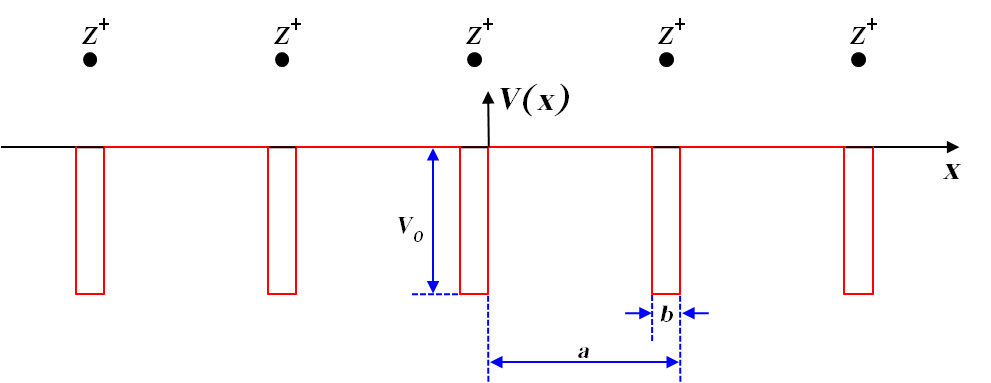
\includegraphics[width=0.75\textwidth]{Periodic_square_potential_130707} 
		\end{figure*}
	 	Then
		\begin{align}
			(A - \lambda I) u_{l} & = \sum_{j \in \N} \left[ (- \frac{d^{2}}{dx^{2}} - \lambda) u_{l}|_{(x_{j}, x_{j+1})} \cdot \mathds{1}_{(x_{j}, x_{j+1})} \right] \label{eq:sepofspectraleq} \\
				& = \sum_{j \in \N} \left[ \left(- \frac{d^{2}}{dx^{2}} - \lambda \right) \left( \eta\left(\frac{|\cdot|}{l}\right) \psi_{s}(\cdot, k) \right)\Big|_{(x_{j}, x_{j+1})} \cdot \mathds{1}_{(x_{j}, x_{j+1})} \right] \notag \\
				& ~\qquad - \frac{2}{l} \sum_{j \in \N} \left[ \left( \eta'\left(\frac{|\cdot|}{l}\right) \psi_{s}'(\cdot, k) \right)\Big|_{(x_{j}, x_{j+1})} \cdot \mathds{1}_{(x_{j}, x_{j+1})}  \right] \notag \\
				& ~\qquad - \frac{1}{l^{2}} \sum_{j \in \N} \left[ \left( \eta''\left(\frac{|\cdot|}{l}\right) \psi_{s}(\cdot, k) \right)\Big|_{(x_{j}, x_{j+1})} \cdot \mathds{1}_{(x_{j}, x_{j+1})} \right] \notag \\
				& = \sum_{j \in \N} \left[ \eta\left(\frac{|\cdot|}{l}\right) \left(- \frac{d^{2}}{dx^{2}} - \lambda \right) \psi_{s}(\cdot, k) |_{(x_{j}, x_{j+1})} \cdot \mathds{1}_{(x_{j}, x_{j+1})} \right] + R \notag
		\end{align}
		where $R$ is a sum of products of derivatives of order $\geq 1$ of $\eta\left(\frac{|\cdot|}{l}\right)$, and derivatives of order $\leq 1$ of $\psi_{s}(\cdot, k)$. Thus, note that $\psi_{s}(\cdot, k) \in H^{2}_{loc}(\R)$, the semi-periodic structure of $\psi_{s}(\cdot, k)$ implies
		\begin{equation}
			 \| R \| \leq \frac{c}{l} \| \psi_{s}(\cdot, k) \|_{H^{1}((x_{0} - \frac{l}{2}, x_{0} + \frac{l}{2}))} \leq c \frac{1}{\sqrt{l}}. \label{eq:estimofR}
		\end{equation}
		Together with \eqref{UIclosed}, \eqref{firstinclusion-firstequation} and \eqref{eq:sepofspectraleq}, this gives
		\[ \frac{1}{\|u_{l}\|}\| (A - \lambda I) u_{l} \| \leq \frac{c}{l} \]
		Now, as moreover $u_{l} \in \mathcal{D}(A)$ this results in
			\[ \frac{1}{\|u_{l} \|} \| (A - \lambda I) u_{l} \| \rightarrow 0 \text{ as } l \rightarrow \infty \]
		Thus, either $\lambda$ is an eigenvalue of $A$, or $(A - \lambda I)^{-1}$ exists but is unbounded. In both cases, $\lambda \in \sigma(A)$.
	\end{proof}
\end{theorem}	

The other inclusion can be shown by simply using the Floquet transformation and the completeness of the Bloch waves. Hence, this prove doesn't differ from the one of any m-th order linear differential operator with periodic coefficients as in \cite[Chapter 3]{Plum10}. Again, due to completeness I still want to list it here.

\begin{theorem} \label{4.1:thm-MainResult.SecondInclusion}

	$\sigma(A) \subset \bigcup_{s \in \N} I_{s}.$

	\begin{proof}
		Let $\lambda \in \R \setminus \bigcup_{s \in \N} I_{s}$. We have to prove that $\lambda \in \rho(A)$, i.e. for each $f \in L^{2}(\R)$ there exists some $u \in \mathcal{D}(A)$ satisfying $(A-\lambda I)u = f$. For given $f \in L^{2}(\R)$, we define, for $l \in \N$, 
			\[ f_{l}(x) \coloneqq \frac{1}{\sqrt{|B|}} \sum_{s=1}^{l} \int_{B} \langle (Uf)(\cdot, k), \psi_{s}(\cdot, k)\rangle_{L^{2}(\Omega)} \psi_{s}(x,k) dk \]
			and
			\begin{equation}
				u_{l} \coloneqq \frac{1}{\sqrt{|B|}} \sum_{s=1}^{l} \int_{B} \frac{1}{\lambda_{s}(k) - \lambda} \langle (Uf)(\cdot, k), \psi_{s}(\cdot, k)\rangle_{L^{2}(\Omega)} \psi_{s}(x, k) dk \label{ul}
			\end{equation} 
		Here, due to \eqref{UIclosed} there exists some $\delta > 0$ such that
			\begin{equation}
				|\lambda_{s}(k) - \lambda| \geq \delta \quad \text{ for all } s \in \N, k \in B \label{lambda-distance}
			\end{equation}

		In particular, consider for fixed $k \in B$ and $v \in \mathcal{D}(A_{k})$:
		\begin{equation}
			(A_{k} - \lambda I) v(\cdot, k) = (Uf)(\cdot, k) \quad \text{ on } \Omega, \label{4.9}			
		\end{equation}
		which has a unique solution as $\lambda \in \R \setminus \bigcup_{s \in \N} I_{s}$. Parseval yields
		\begin{align*}
			\| (Uf)(\cdot, k)\|^{2}_{L^{2}(\Omega)} & = \sum_{s=1}^{\infty} |\langle (Uf)(\cdot, k), \psi_{s}(\cdot, k)\rangle|^{2} \\
			& = \sum_{s=1}^{\infty}|\langle (A - \lambda) v(\cdot, k), \psi_{s}(\cdot, k)\rangle_{L^{2}(\Omega)}|^{2}
		\end{align*}

		Since both $v(\cdot, k)$ and $\psi_{s}(\cdot, k)$ satisfy semi-periodic boundary conditions, $A - \lambda I$ can be moved to $\psi_{s}(\cdot, k)$ in the inner product, and hence \eqref{eigv-problem} and \eqref{lambda-distance} give
		\begin{align*}
			\| (Uf)(\cdot,k)\|^{2}_{L^{2}(\Omega)} & = \sum_{s=1}^{\infty} |\lambda_{s}(k) - \lambda|^{2} |\langle v(\cdot, k), \psi_{s}(\cdot, k)\rangle_{L^{2}(\Omega)}|^{2} \\
			& \geq \delta^{2} \| v(\cdot, k)\|^{2}_{L^{2}(\Omega)}.
		\end{align*}
		By Theorem \ref{3.2:thm-UIsometricIsomorphism}, this implies $v \in L^{2}(\Omega \times B)$, and we can define $u \coloneqq U^{-1} v \in L^{2}(\R)$. Thus, \eqref{4.9} gives
			\begin{align*}
				\langle (Uf)(\cdot, k), \psi_{s}(\cdot, k) \rangle_{L^{2}(\Omega)} & = \langle (A - \lambda I)(Uu)(\cdot, k), \psi_{s}(\cdot, k) \rangle_{L^{2}(\Omega)} \\
					& = \langle (Uu)(\cdot,k), (A - \lambda I) \psi_{s}(\cdot, k) \rangle_{L^{2}(\Omega)} \\
					& = (\lambda_{s}(k) - \lambda) \langle Uu(\cdot, k), \psi_{s}(\cdot, k) \rangle_{L^{2}(\Omega)}
			\end{align*}
		whence \eqref{ul} implies
			\[ u_{l}(x) = \frac{1}{\sqrt{|B|}} \sum_{s=1}^{l} \int \langle (Uu)(\cdot, k), \psi_{s}(\cdot, k)\rangle_{L^{2}(\Omega)} \psi_{s}(x, k) dk, \]
		and Theorem \ref{3.3:thm-flConvergence} gives
			\begin{equation}
				u_{l} \rightarrow u, \quad f_{l} \rightarrow f \quad \text{ in } L^{2}(\R). \label{ulflconvergence}
			\end{equation}
		We will now prove that
		\begin{equation}
				(A - \lambda I) u_{l} = f_{l} \text{ for all } l \in \N \label{lefttoprove}
			\end{equation} 
		which implies that $\langle u_{l}, (A - \lambda I) v \rangle = \langle f_{l}, v\rangle$ for all $v \in \mathcal{D}(A)$, whence Theorem \ref{3.16} implies $u_{l} \in \mathcal{D}(A)$, and
			\[ (A - \lambda I) u_{l} = f_{l} \quad \text{ for all } l \in \N \]
		Since $A$ is closed, \eqref{ulflconvergence} now implies
			\[ u \in \mathcal{D}(A) \text{ and } (A - \lambda I) u = f \]
		which is the desired result.
		
		We are left to prove is \eqref{lefttoprove}, i.e. that
			\begin{equation}
				\langle u_{l} , (A - \lambda I) \varphi \rangle_{L^{2}(\R)} = \langle f_{l},\varphi \rangle_{L^{2}(\R)} \quad \forall \varphi \in C_{0}^{\infty}(\R). \label{lefttoshow2}
			\end{equation} 
		So, let $\varphi \in C_{0}^{\infty}(\R)$ be fixed, and let $K \subseteq \R$ denote an open interval containing $\supp(\varphi)$ in its interior. Both the functions
		\begin{align*}
			r_{s}(x, k) & \coloneqq \frac{1}{\lambda_{s}(k) - \lambda} \langle (Uf)(\cdot, k), \psi_{s}(\cdot, k) \rangle_{L^{2}(\Omega)} \psi_{s}(x, k) \overline{(A - \lambda I) \varphi(x)}, \\
			t_{s}(x, k) & \coloneqq \langle (Uf)(\cdot, k), \psi_{s}(\cdot, k) \rangle_{L^{2}(\Omega)} \psi_{s}(x, k) \overline{\varphi(x)}
		\end{align*}
		are in $L^{2}(K \times B)$ by Fubini's Theorem, since \eqref{lambda-distance} and the fact that $(A_{k} - \lambda I) \varphi \in L^{\infty}(K)$ and $\varphi \in L^{\infty}(K)$, imply both
		\begin{align*}
			\| r_{s} \|_{L^{2}(K \times B)} & \leq c \| (Uf)(\cdot, k) \|^{2}_{L^{2}(\Omega)} \| \psi_{s}(\cdot, k) \|^{2}_{L^{2}(K)} 
		\intertext{and}
			\| t_{s} \|_{L^{2}(K \times B)} & \leq \tilde{c} \| (Uf)(\cdot, k) \|^{2}_{L^{2}(\Omega)} \| \psi_{s}(\cdot, k) \|^{2}_{L^{2}(K)},.			
		\end{align*}
		the latter factor is bounded as a function of $k$ because $K$ is covered by a finite number of copies of $\Omega$, and the former is in $L^{1}(B)$ by Theorem \ref{3.2:thm-UIsometricIsomorphism}.
		
		Since $K \times B$ is bounded, $r$ and $t$ are also in $L^{1}(K \times B)$. Therefore, Fubini’s Theorem implies that the order of integration with respect to $x$ and $l$ may be exchanged for $r$ and $t$. Thus, by \eqref{ul},
			\begin{align*}
				\int_{K} u_{l}(x) \overline{(A - \lambda I) \varphi(x)} dx & = \frac{1}{\sqrt{|B|}} \sum_{s=1}^{l} \int_{K} \left( \int_{B} r_{s}(x, k) dk \right) dx \\
					& = \frac{1}{\sqrt{|B|}} \sum_{s=1}^{l} \int_{B} \frac{1}{\lambda_{s}(k) - \lambda} \langle (Uf)(\cdot, k), \psi_{s}(\cdot, k) \rangle_{L^{2}(\Omega)} \\
					& ~\qquad ~\qquad ~\qquad ~\qquad \langle \psi_{s}(\cdot, k), (A - \lambda I) \varphi \rangle_{L^{2}(K)} dk. 
			\end{align*}
			Since $\varphi$ has compact support in the interior of $K$, $(A - \lambda I)$ may be moved to $\psi_{s}(\cdot, k)$, and hence \eqref{eigv-problem} gives
			\begin{align*}
				\int_{K} u_{l}(x) \overline{(A - \lambda I) \varphi(x)} dx					& = \frac{1}{\sqrt{|B|}} \sum_{s=1}^{l} \int_{B} \langle (Uf)(\cdot, k), \psi_{s}(\cdot, k) \rangle_{L^{2}(\Omega)} \langle \psi_{s}(\cdot, k), \varphi \rangle_{L^{2}(K)} dk \\
				 	& = \frac{1}{\sqrt{|B|}} \sum_{s=1}^{l} \int_{B} \left( \int_{K} t_{s}(x, k) dx \right) dk \\
					& = \int_{K} \left[ \frac{1}{\sqrt{|B|}} \sum_{s=1}^{l} \int_{B} \langle (Uf)(\cdot, k), \psi_{s}(\cdot, k) \rangle_{L^{2}(\Omega)} \psi_{s}(x, k) dk \right] \overline{\varphi(x)} dx \\
					& = \int_{K} f_{l}(x) \overline{\varphi(x)} dx,
			\end{align*}
			i.e. \eqref{lefttoshow2}.
	\end{proof}
\end{theorem}